
\chapter{Verification}

The terms {\em verification} and {\em validation} are often used interchangeably to mean the process of checking the accuracy of a numerical model. For many, this entails comparing model predictions with experimental measurements. However, there is now a fairly broad-based consensus that comparing model and experiment is largely what is considered {\em validation}. So what is {\em verification}? ASTM~E~1355~\cite{ASTM:E1355}, ``Standard Guide for Evaluating the Predictive Capability of Deterministic Fire Models,'' defines verification as
\begin{quote}
The process of determining that the implementation of a calculation method accurately represents the developer's conceptual description of the calculation method and the solution to the calculation method.
\end{quote}
and it defines validation as
\begin{quote}
The process of determining the degree to which a calculation method is an accurate representation of the real world from the perspective of the intended uses of the calculation method.
\end{quote}
Simply put, verification is a check of the math; validation is a check of the physics. If the model predictions closely match the results of experiments, using whatever metric is appropriate, it is assumed by most that the model suitably describes, via its mathematical equations, what is happening. It is also assumed that the solution of these equations must be correct. So why do we need to perform model verification? Why not just skip to validation and be done with it? The reason is that rarely do model and measurement agree so well in all applications that anyone would just accept its results unquestionably. Because there is inevitably differences between model and experiment, we need to know if these differences are due to limitations or errors in the numerical solution, or the physical sub-models, or both.

Whereas model validation consists mainly of comparing predictions with experimental measurements, as documented later in this guide, model verification consists of a much broader range of activities, from checking the computer program itself, to comparing calculations to analytical (exact) solutions, to understanding the impact on model outputs from a range of different model inputs.

A series of verification test cases follow, examining the energy balance, mass balance, ventilation, heat transfer and sprinkler effects modeled by CFAST. These test cases are routinely run to ensure the calculations in the model are correct for a range of simple calculations where analytical solutions exist. The energy and mass balance examples test the underlying fundamental equations that determine conditions within a compartment in the model. The ventilation examples test the flow of gases between compartments through doors, windows, holes in floors/ceilings, and mechanical ventilation systems.  The heat transfer examples test the flow of energy through walls of compartments or to user-defined objects within a compartment. The sprinkler example tests the algorithm used to simulate the response of heat detectors and fire sprinklers in CFAST.  For each of the examples, an analytical solution is presented and compared to the results of a matching CFAST simulation.


\section{Energy Balance}

For most of the examples presented in this section, the same basic geometry is used, a single 5~m by 5~m by 5~m compartment.

\subsection{Temperature Equilibrium via Heat Conduction}

As a simple test of the energy balance, raising the external temperature of the base case compartment from an initial condition of 20~\degc to 25~\degc allows the internal temperature to equilibrate to the exterior. From the ideal gas law, the pressure inside the compartment is expected to rise to
\begin{equation}
   P_{\rm final} = P_{\rm initial} \; \frac{T_{\rm final}}{T_{\rm initial}} = 101325 \; {\rm Pa} \times \frac{298.15 \; {\rm K}}{293.15 \; {\rm K}} = 103053 \; {\rm Pa} \label{eq:Temperature_Equilibrium}
\end{equation}
or a final pressure rise of 1728 Pa.  Figure \ref{fig:Temperature_Equilibrium} shows the simulated conditions for this test, which are consistent with the expected results..

\begin{figure}[!ht]
\begin{tabular*}{\textwidth}{l@{\extracolsep{\fill}}r}
\includegraphics[width=3.0in]{SCRIPT_FIGURES/Verification/basic_tempequilib_temp} &
\includegraphics[width=3.0in]{SCRIPT_FIGURES/Verification/basic_tempequilib_pres}
\end{tabular*}
\caption[Results of the test case {\ct basic\_tempequilib.in}]{Interior temperature and pressure in equilibrium with the exterior in the case {\ct basic\_tempequilib.in}.}
\label{fig:Temperature_Equilibrium}
\end{figure}

\subsection{Temperature Equilibrium via a Window}

Now an open window is added to the compartment, with an exterior temperature of 25~\degc. Figure~\ref{fig:Temperature_Equilibrium_With_Window} shows the interior conditions coming into equilibrium with the exterior, which are consistent with the expected results..

\begin{figure}[!ht]
\begin{tabular*}{\textwidth}{l@{\extracolsep{\fill}}r}
\includegraphics[width=3.0in]{SCRIPT_FIGURES/Verification/basic_tempequilib_window_temp} &
\includegraphics[width=3.0in]{SCRIPT_FIGURES/Verification/basic_tempequilib_window_pres}
\end{tabular*}
\caption[Results of the test case {\ct basic\_tempequilib\_window.in}]{Interior temperature and pressure in equilibrium with the exterior in the case {\ct basic\_tempequilib\_window.in}.}
\label{fig:Temperature_Equilibrium_With_Window}
\end{figure}

\subsection{Temperature Equilibrium via a Window at a High Elevation}

With the exterior temperature still set to 25~\degc, the elevation is raised to 1500~m, approximately the average elevation of Idaho.  Since CFAST calculations are relative to the exterior ambient, conditions are expected to be identical to the previous examples and equilibrate to those of the exterior. Figure \ref{fig:Temperature_Equilibrium_Elevation} shows the simulated conditions for the test case, which are consistent with the expected results..

\begin{figure}[!ht]
\begin{tabular*}{\textwidth}{l@{\extracolsep{\fill}}r}
\includegraphics[width=3.0in]{SCRIPT_FIGURES/Verification/basic_tempequilib_window_elevation_temp} &
\includegraphics[width=3.0in]{SCRIPT_FIGURES/Verification/basic_tempequilib_window_elevation_pres}
\end{tabular*}
\caption[Results of the test case {\ct basic\_tempequilib\_window\_elevation.in}]{Interior temperature and pressure in equilibrium with the exterior in the case {\ct basic\_tempequilib\_window\_elevation.in}.}
\label{fig:Temperature_Equilibrium_Elevation}
\end{figure}


\clearpage

\section{Mass Balance}

\label{mass_conservation}
\subsection{A Fire in a Single, Sealed Compartment}
\label{sec:spec1}
A methane fire burns in a sealed compartment of dimension 5~m by 6~m by 3~m. The heat release rate ramps up linearly to 1~kW in 30~s, then remains steady for 5~min, and then ramps down linearly to 0 in 30~s. The total energy released is 330~kJ, and the total mass of fuel consumed is
\begin{equation}
  \frac{ 330 \; {\rm kJ} }{ 50000 \; {\rm kJ/kg} } = 0.00660 \; {\rm kg}
\end{equation}
where the heat of combustion of methane is taken to be 50 000 kJ/kg. For complete combustion of methane, the combustion chemistry is given by
\begin{equation}
   \mathrm{CH_4 + 2 \, O_2 \to CO_2 + 2 \, H_2O}
   \label{eq:Methane_Combustion}
\end{equation}
The molecular weight of CH$_4$ is 16~g/mol and CO$_2$ is 44~g/mol; thus, the total mass of CO$_2$ produced by the fire is
\begin{equation}
   m_{\rm CO_2} = 0.0066 \; {\rm kg} \times  \frac{ 44 \; {\rm g/mol} }{ 16 \; {\rm g/mol} } = 0.01815 \; {\rm kg}
\end{equation}
The molecular weight of H$_2$O is 18~g/mol; thus, the total mass of H$_2$O produced by the fire is
\begin{equation}
   m_{\rm H_2O} = 0.0066 \; {\rm kg} \times  \frac{ 2(18) \; {\rm g/mol} }{ 16 \; {\rm g/mol} } = 0.01485 \; {\rm kg}
\end{equation}
CFAST predicts that the final mole fractions of O$_2$, CO$_2$ and H$_2$O in the upper layer are 0.2069, 0.00012 and 0.00024, respectively (calculated by the model consistent with eq. \ref{eq:Methane_Combustion}; see \cite{CFAST_Tech_Guide_7} for details of the combustion chemistry calculations in CFAST). The remainder is N$_2$, whose mole fraction is 0.7927. These mole fractions can be converted to mass fractions by
\begin{equation}
Y_k = \frac{X_{k} M_{k}}{\sum_{i=1}^N X_{i}M_{i}}
\end{equation}
The mass of the upper layer can be calculated from the equation of state:
\begin{equation}
m_{\rm u} = \frac{P \, V}{R \, T} \quad ; \quad R = \frac{\gamma-1}{\gamma} \, c_p \approx 289.14 \; {\rm  \frac{J}{kg \cdot K}}
\end{equation}
The mass of CO$_2$ and H$_2$O produced is given by
\begin{equation}
m_{k} = m_{\rm u} \, Y_{k}
\end{equation}
Figure~\ref{specmass1} shows the resulting product masses, which are consistent with the expected results.

\begin{figure}[!ht]
\centering
\includegraphics[width=3.0in]{SCRIPT_FIGURES/Verification/species_mass_1}
\caption[Results of the test case {\ct species\_mass\_1.in}]{Expected and predicted masses of CO$_2$ and H$_2$O for the case {\ct species\_mass\_1.in}.}
\label{specmass1}
\end{figure}


\subsection{A Fire in a Compartment Connected to Another via a Door}
\label{sec:spec2}

The same natural gas fire described in Section~\ref{sec:spec1} burns in a compartment of dimension 2~m by 5~m by 8~m which is connected to another compartment of dimension 5~m by 3~m by 8~m. A doorway connects the compartments, which has a width of 1~m and a height of 6~m. Because the fire and the fuel source have not changed, the theoretical calculations for the mass of CO$_2$ and H$_2$O produced will remain the same. The remaining portion of the problem is approached in the same manner, but since there are two compartments, the mass of CO$_2$ and H$_2$O produced in each layer of each compartment must be individually calculated and then summed together to produce the net yields of CO$_2$ and H$_2$O. Figure~\ref{specmass2} shows the resulting product masses, which are consistent with the expected results.
\begin{figure}[!ht]
\centering
\includegraphics[width=3.0in]{SCRIPT_FIGURES/Verification/species_mass_2}
\caption[Results of the test case {\ct species\_mass\_1.in}]{Expected and predicted masses of CO$_2$ and H$_2$O for the case {\ct species\_mass\_2.in}.}
\label{specmass2}
\end{figure}

\subsection{A Fire in a Compartment Connected to Another via a Ceiling Vent}

The same natural gas fire described in Section~\ref{sec:spec1} burns in a compartment of dimension 9~m by 5~m by 4~m which is connected to another compartment of dimension 9~m by 5~m by 2~m. The compartments are placed such that the second one is located directly above the first one. There is a square ceiling vent between the compartments that has an area of 4~m$^2$. This problem is approached in the same exact manner as in Section~\ref{sec:spec2} because the only difference between the two scenarios is the specific alignment of the compartments.
Figure~\ref{specmass2} shows the resulting product masses, which are consistent with the expected results.
\begin{figure}[!ht]
\centering
\includegraphics[width=3.0in]{SCRIPT_FIGURES/Verification/species_mass_3}
\caption[Results of the test case {\ct species\_mass\_3.in}]{Expected and predicted masses of CO$_2$ and H$_2$O for the case {\ct species\_mass\_3.in}.}
\label{specmass3}
\end{figure}

\subsection{A Fire in a Four Compartment Assembly}
\label{sec:specmass4}

Four 4~m by 4~m by 4~m compartments are arranged such that two compartments are placed adjacent to one another and the following two compartments are placed directly on top of the first two. The same natural gas fire described in Section~\ref{sec:spec1} burns in the first compartment of this setup. After 2500~s, the wall between compartments one and two is removed, forcing the gases in the two rooms to mix. Next, at 5000~s, the wall between compartments three and four is removed. Lastly, at 7500~s, the ceiling of compartment four is removed, allowing the system to slowly return to ambient conditions. Figure~\ref{fig:specmass4ab} and Figure~\ref{fig:specmass4cd} show how the masses of CO$_2$ and H$_2$O in each compartment change with respect to time. Figure~\ref{fig:specmass4TP} shows that the expected temperature and pressure values of compartment one are consistent with the values produced by CFAST.

\begin{figure}[!ht]
\begin{tabular*}{\textwidth}{l@{\extracolsep{\fill}}r}
\includegraphics[width=3.0in]{SCRIPT_FIGURES/Verification/species_mass_4a} &
\includegraphics[width=3.0in]{SCRIPT_FIGURES/Verification/species_mass_4b}
\end{tabular*}
\caption[Results of the test case {\ct species\_mass\_4.in}]{Expected and CFAST calculated values for the masses of CO$_2$ and H$_2$O in compartments one and two for case {\ct species\_mass\_4.in}.}
\label{fig:specmass4ab}
\end{figure}

\begin{figure}[!ht]
\begin{tabular*}{\textwidth}{l@{\extracolsep{\fill}}r}
\includegraphics[width=3.0in]{SCRIPT_FIGURES/Verification/species_mass_4c} &
\includegraphics[width=3.0in]{SCRIPT_FIGURES/Verification/species_mass_4d}
\end{tabular*}
\caption[Results of the test case {\ct species\_mass\_4.in}]{Expected and CFAST calculated values for the masses of CO$_2$ and H$_2$O in compartments three and four for case {\ct species\_mass\_4.in}.}
\label{fig:specmass4cd}
\end{figure}

\begin{figure}[!ht]
\begin{tabular*}{\textwidth}{l@{\extracolsep{\fill}}r}
\includegraphics[width=3.0in]{SCRIPT_FIGURES/Verification/species_mass_4_temperature} &
\includegraphics[width=3.0in]{SCRIPT_FIGURES/Verification/species_mass_4_pressure}
\end{tabular*}
\caption[Results of the test case {\ct species\_mass\_4.in}]{Expected and CFAST calculated values for pressure and temperature of the first compartment for the case {\ct species\_mass\_4.in}.}
\label{fig:specmass4TP}
\end{figure}

\clearpage


\section{Energy Balance}

\subsection{A Fire in a Single, Sealed Compartment with a Single Zone}
\label{sealed_test}

A 100~kW methane fire burns in a sealed compartment with no ventilation, adiabatic walls, and no radiative emission. A single zone simulation is run in which it is assumed that the entire volume is taken up by the upper layer.  From Eqs. (2.5) and (2.6) in the CFAST Technical Guide~\cite{CFAST_Tech_Guide_6}, the governing equation for the pressure and temperature of the single zone compartment are:
\begin{eqnarray}
   \frac{{\rm d} P}{{\rm d}t} &=& \frac{\gamma-1}{V} \, \dot{q}   \label{eq1}
 \\[0.1in]
   \frac{{\rm d} T}{{\rm d}t} &=& \frac{1}{c_p \, m} \left( \dot{q} - c_p \, \dot{m} \, T + V \, \frac{{\rm d} P}{{\rm d}t} \right)
   \label{eq2}
\end{eqnarray}
where $m$ is the total mass in the volume, $\dot{m}=\dm_{\rm f}$ is the mass flow rate of the fuel into the volume, and
$\dot{q}=\dot{Q} + c_p \, \dot{m}_{\rm f} \, T_{\rm f} $ is the heat release rate of the fire plus the heat flow rate of the fuel flowing into the volume.
Note that $\dot{m}$ and $\dot{q}$ are source terms, they are assumed to have this form for this test problem.

Eq.~(\ref{eq2}) can be shown to be equivalent to the first law of thermodynamics by first substituting ${\rm d}P/{\rm d}t$ from Eq.~(\ref{eq1}) and noting that $\gamma=c_p/c_v$ to obtain
\begin{eqnarray}
   \frac{{\rm d} T}{{\rm d}t} &=& \frac{1}{c_p \, m} \left( \dot{q} - c_p \, \dot{m} \, T +  (\gamma-1) \, \dot{q}\right)\\
   \label{eq3}
    &=& \frac{1}{c_p \, m} \left( \gamma\dot{q} - c_p \, \dot{m} \, T   \right)\\
    &=& \frac{1}{c_v \, m} \left( \dot{q} - c_v \, \dot{m} \, T   \right)\label{eq4}
\end{eqnarray}

\noindent Next, the first law of thermodynamics can be stated as
\begin{eqnarray}
\frac{\rm d}{{\rm d}t}\left(c_vmT\right) = \dot{q} - P\frac{{\rm d}V}{{\rm d}t}=\dot{q}\label{eq5}
\end{eqnarray}
since ${\rm d}V/{\rm d}t=0$ (for this case).
\noindent Expanding and solving for ${\rm d} T/{\rm d}t$ results in
\begin{eqnarray}
c_v\dot{m}T+c_vm\frac{{\rm d}T}{{\rm d}t} &= &\dot{q}\\
    \frac{{\rm d} T}{{\rm d}t}&=& \frac{1}{c_v \, m} \left( \dot{q} - c_v \, \dot{m} \, T   \right)
\end{eqnarray}
which is identical Eq.~(\ref{eq4}) and therefore equivalent to Eq.~(\ref{eq2}).

Since the right hand side of Eq.~(\ref{eq1}) is constant, it may be integrated to obtain the solution
\begin{equation}
P(t)=P_0+\frac{\gamma-1}{V}\,\dot{q}\,t \label{eq:soleq1}
\end{equation}
where $P_0$ is the initial pressure.  A solution for Eq.~(\ref{eq2}) may be found by using Eq.~(\ref{eq:soleq1}) and the ideal gas law to obtain
\begin{equation}
T(t)=\frac{V\,P(t)}{R\,m(t)}\label{eq:soleq2}
\end{equation}
where $m(t)=m_0+\dot{m}\,t$, $m_0=\frac{P_0\,V}{R\,T_0}$, is the initial mass, $T_0$ is the initial pressure and $R=c_p-c_v$.

Figure~\ref{fig:Analytical_Closed_Compartment} includes comparisons of the temperature and pressure as predicted by CFAST and the analytic solutions given
in Eqs.~(\ref{eq:soleq1}) and (\ref{eq:soleq2}).

\begin{figure}[!ht]
\begin{tabular*}{\textwidth}{l@{\extracolsep{\fill}}r}
\includegraphics[width=3.0in]{SCRIPT_FIGURES/Verification/sealed_test_temp} &
\includegraphics[width=3.0in]{SCRIPT_FIGURES/Verification/sealed_test_pres}
\end{tabular*}
\caption[Results of the test case {\ct sealed\_test.in}]{Temperature and pressure rise due to a fire in a closed compartment. The case is called {\ct sealed\_test.in}.}
\label{fig:Analytical_Closed_Compartment}
\end{figure}

\subsection{A Fire in a Single, Sealed Compartment with Two Zones}

Consider now the same case as in Section~\ref{sealed_test}, but now with two zones rather than one. The compartment pressure ought to be the same as before, and the upper layer temperature ought to converge to the single layer temperature as seen in Fig.~\ref{fig:Analytical_Closed_Compartment2}.
\begin{figure}[!ht]
\begin{tabular*}{\textwidth}{l@{\extracolsep{\fill}}r}
\includegraphics[width=3.0in]{SCRIPT_FIGURES/Verification/sealed_test_2_layers_temp} &
\includegraphics[width=3.0in]{SCRIPT_FIGURES/Verification/sealed_test_2_layers_pres}
\end{tabular*}
\caption[Results of the test case {\ct sealed\_test\_2\_layers.in}]{Hot gas layer temperature and pressure rise due to a fire in a closed compartment with two zones. The case is called {\ct sealed\_test\_2\_layers.in}.}
\label{fig:Analytical_Closed_Compartment2}
\end{figure}

\clearpage


\section{Ventilation}

\subsection{Pressure Change as Air Flows Through a Single Compartment}
The setup for this test case includes a 5~m by 5~m by 3~m compartment that contains a mechanical vent and a wall vent. Air is pumped into a single compartment through a 1~m by 1~m mechanical vent, at a rate of 0.01~m$^3$/s. The air is allowed to exit the compartment through a 1~cm by 1~cm vent located on the opposite side of the compartment. The governing equation for the change in pressure in the compartment is \cite{Emmons:SFPE}:
\begin{equation}
\Delta{P} = \frac{1}{2\rho}\brackets{\frac{\dot{m}}{CA}}^2
\end{equation}
where $\rho$ , $\dot{m}$ and $C$ are consistent with CFAST calculations
\begin{equation}
\rho = \frac{P}{RT} \quad ; \quad  \dot{m} = \rho_{\infty} \dot{V} \quad ; \quad C = 0.70
\end{equation}
Figure~\ref{fig:vent1} shows how the pressure changes as air flows through the compartment.

\begin{figure}[!ht]
\centering
\includegraphics[width=3.0in]{SCRIPT_FIGURES/Verification/ventilation_1_pressure}
\caption[Results of the test case {\ct ventilation\_1.in}]{Expected and CFAST calculated values for pressure of the compartment for the case {\ct ventilation\_1.in}.}
\label{fig:vent1}
\end{figure}



\subsection{Temperature and Pressure Changes of Steady-State Air Flow}
\label{sec:vent2}

A similar setup to the one used in Section~\ref{sec:specmass4} is employed here. A fan blows air into the first compartment, on the ground floor, at a rate of 1~m$^3$/s and then continues to the second compartment after passing through a doorway. The air then travels to the third compartment by passing through a ceiling vent with an area of 3~m$^2$ and continues to compartment four through another doorway. Air is finally extracted from compartment four at a rate of 1~m$^3$/s. Figure~\ref{ventilation_2TP} shows how temperature and pressure change as the air flows through the fourth compartment.

\begin{figure}[!ht]
\begin{tabular*}{\textwidth}{l@{\extracolsep{\fill}}r}
\includegraphics[width=3.0in]{SCRIPT_FIGURES/Verification/ventilation_2_temperature} &
\includegraphics[width=3.0in]{SCRIPT_FIGURES/Verification/ventilation_2_pressure}
\end{tabular*}
\caption[Results of the test case {\ct ventilation\_2.in}]{Expected and CFAST calculated values for pressure and temperature of the fourth compartment for the case {\ct ventilation\_2.in}.}
\label{ventilation_2TP}
\end{figure}


\subsection{Temperature and Pressure Changes of Non Steady-State Air Flow}

The same setup that was constructed in Section~\ref{sec:vent2} is used again in this scenario. All vents and fans are the same as in the previous case, except the fan in the fourth compartment has been converted to a round ceiling vent with an area of 4~m$^2$. Initially, all of the vents are closed and air is pumped into the first compartment at a rate of 1~m$^3$/s, for a period of 15~s. After 15~s pass, the fan is shut off. Then, at 200~s, the door between compartments one and two opens completely. Next, at 500~s, the vent between compartments two and three opens completely. At 700~s, the door between compartments three and four opens completely. Finally, at 1000~s, the ceiling vent in compartment four opens completely. Figure~\ref{ventilation_3TP} shows how temperature and pressure change as the air flows through the first compartment.

\begin{figure}[!ht]
\begin{tabular*}{\textwidth}{l@{\extracolsep{\fill}}r}
\includegraphics[width=3.0in]{SCRIPT_FIGURES/Verification/ventilation_3_temperature} &
\includegraphics[width=3.0in]{SCRIPT_FIGURES/Verification/ventilation_3_pressure}
\end{tabular*}
\caption[Results of the test case {\ct ventilation\_3.in}]{Expected and CFAST calculated values for pressure and temperature of the first compartment for the case {\ct ventilation\_3.in}.}
\label{ventilation_3TP}
\end{figure}

\subsection{Determining the Velocity Profile of Air Flowing Through a Doorway}

A 200~kW natural gas (methane) fire burns in a 5~m by 5~m by 5~m compartment, where the walls are assumed to be adiabatic. The heat release rate ramps up linearly to 200~kW in 30~s, then remains steady for 5.5~min. The compartment contains a 4~m by 1.5~m door that remains completely open throughout the simulation. The mass flow though each vertical segment of the doorway is given by:
\begin{equation}
\dot{m} = \int_b^t C \sqrt{2\rho\Delta{P(z)}} \, w\;\mathrm{d}z
\label{eq:mdot}
\end{equation}
where $C$ is the orifice coefficient taken to be 0.7, $\rho$ is the gas density of the upwind compartment, $w$ is the width of the doorway and $\Delta{P(z)}$ is the pressure across the interface at elevation $z$. Finally, $z = b$ and $z = t$ refer to the heights of the bottom and top of the vertical segment in the doorway through which the mass flow rate is being calculated. This equation can be analytically integrated to yield:
\begin{equation}
\dot{m} = {\rm sign} \brackets{\frac{\Delta P_t + \Delta P_b}{2}} \, \frac{2}{3} \, C \sqrt{2\rho} \, w \, (t-b)\frac{|\Delta P_t|^{3/2}-|\Delta P_b|^{3/2}}{|\Delta P_t|-|\Delta P_b|}
\end{equation}
The equation for the velocity profile of air traveling through the doorway can be produced after rearranging equation~\ref{eq:mdot}:
\begin{equation}
v(z) = \frac{\dot{m}}{\delta A \, \rho} = {\rm sign}(\Delta{P(z)}) \, C \sqrt{\frac{2|\Delta{P(z)}|}{\rho}}
\end{equation}
where $\delta A$ represents the infinitesimal area of the door segment and $\rho$ corresponds to the density of air at height $z$. Figure~\ref{fig:vel} shows how the velocity of air flowing through the doorway changes from the floor to the top of the doorway.

\begin{figure}[!ht]
\centering
\includegraphics[width=3.0in]{SCRIPT_FIGURES/Verification/ventilation_4_vel}
\caption[Results of the test case {\ct ventilation\_4.in}]{CFAST calculated velocity profile of air traveling through the doorway in test case {\ct ventilation\_4.in}.}
\label{fig:vel}
\end{figure}

\subsection{Mass Flow Through Different Vent Types}

A fan is supplies air into a compartment at a constant rate of 0.1 m$^3$/s (0.12 kg/s). Vertical and horizontal natural flow vents connect this compartment to two other compartments stacked vertically.  Finally, the structure is vented to the outside by either a vertical or horizontal flow vent in the rooms removed from the one where air is supplied. Figure~\ref{fig:vvent} shows a sample of the mass flow through the vents.

\begin{figure}
\begin{center}
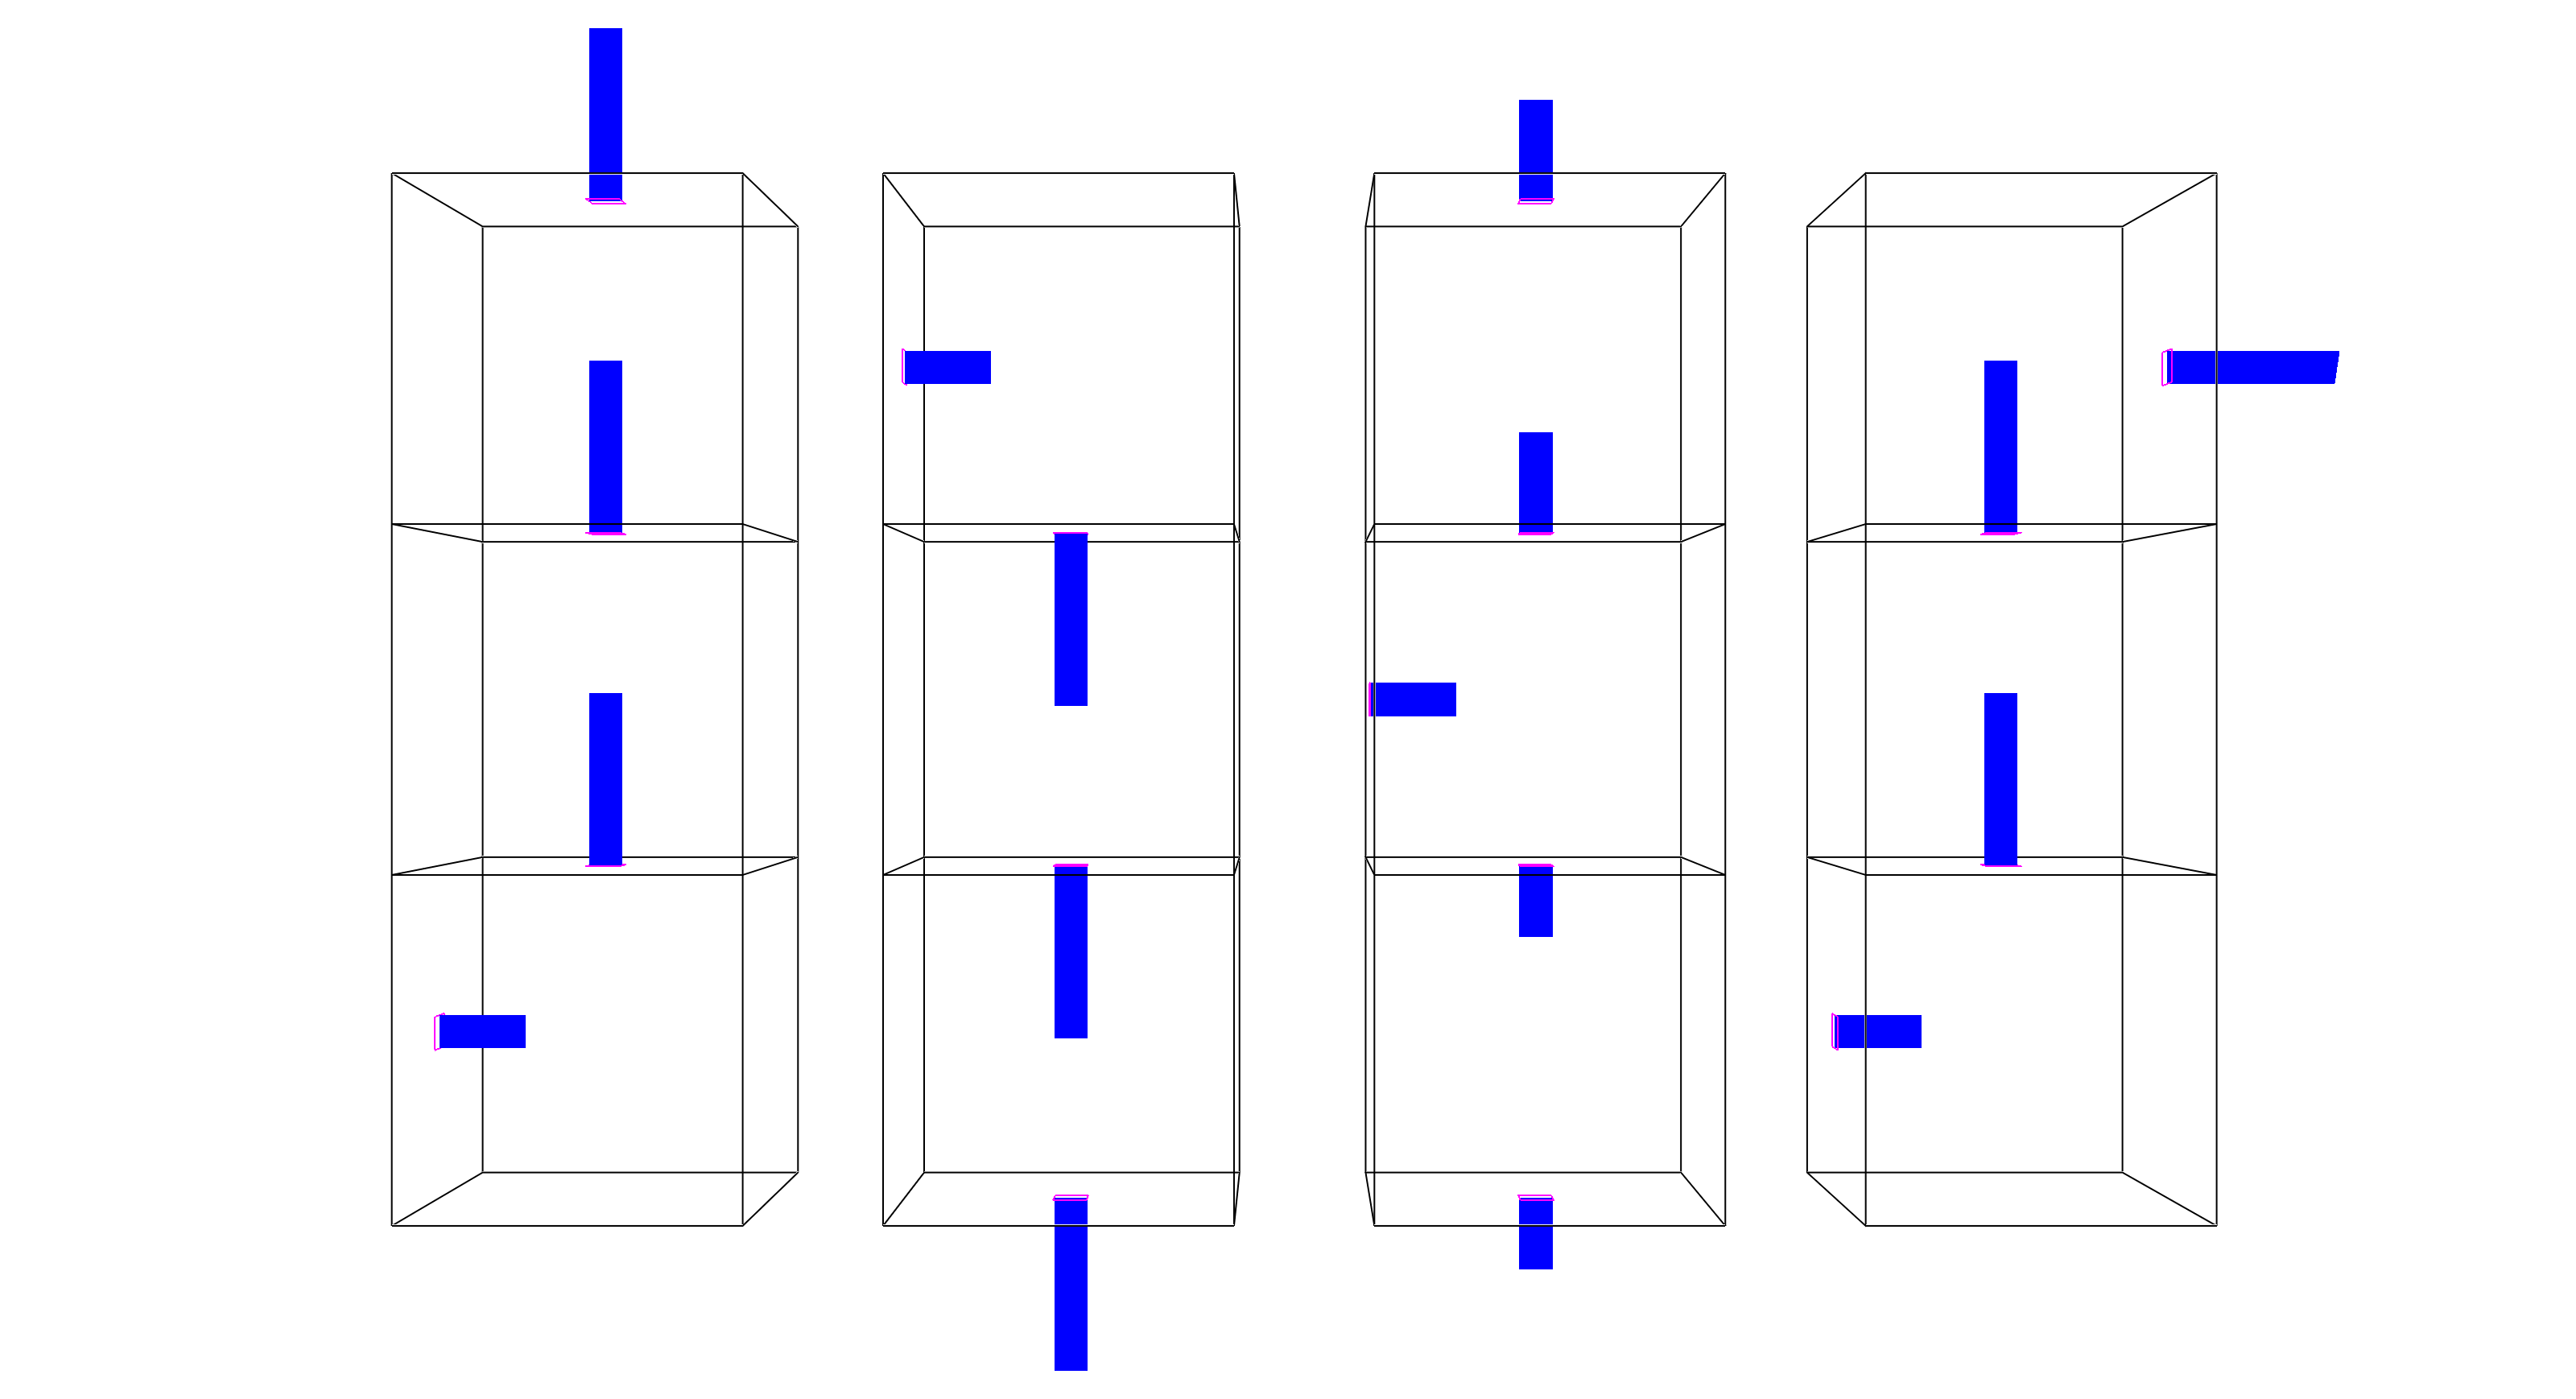
\includegraphics[height=3.0in]{FIGURES/Verification/VVent_Geom} \\
\includegraphics[width=3.0in]{SCRIPT_FIGURES/Verification/VVent_Tests}
\end{center}
\caption[Results of the test case {\ct VVent\_Tests.in}]{Expected and CFAST calculated values for mass flow through vents {\ct VVent\_Tests.in}.}
\label{fig:vvent}
\end{figure}

\section{Heat Transfer}

\subsection{Measuring the Temperature Change of a Thermally Thin Target}

A constant 10~kW natural gas (methane) fire burns in the center of a 15~m by 15~m by 15~m compartment. Because the purpose of this case is to test the point source radiation model and the heating of a thermally-thin target, there is a 20~m$^2$ vent located in the center of the ceiling to exhaust the smoke from the fire and maintain an ambient temperature lower layer. A 1.5~mm thick sheet of plain carbon steel is placed 2~m to the right of the fire. It is oriented directly at the fire. The target is heated by the thermal radiation from the fire, and it is cooled via convective and radiative loss. The net radiative heat transfer to the target is given by:
\begin{equation}
\dqr'' = \epsilon \frac{\chi_{\rm r} \, \dot{Q}}{4\pi \, r^2} + 2\epsilon \sigma ( T_{\rm g}^4 - T_{\rm s}^4)
\end{equation}
where $\epsilon$ is the emissivity of the target, $\chi_{\rm r}$ represents the radiative heat fraction of the fire, $\dot{Q}$ is the heat release rate of the fire, $r$ is the distance between the fire and the target and $\sigma$ is the Stefan-Boltzmann constant, which has a value of $5.67 \times 10^{-11}$~kW/(m$^2 \cdot$K$^4$). Additionally, $T_{\rm g}$ is the temperature of the gas surrounding the target and $T_{\rm s}$ is the temperature of the target's surface. The convective heat flux to a solid surface is governed by the following equations:
\begin{equation}
\dqc'' = h(T_{\rm g}-T_{\rm s}) \quad ; \quad  h = C|T_{\rm g} - T_{\rm s}|^{1/3}
\end{equation}
where $h$ is the convective heat transfer coefficient and $C$ is an empirical coefficient determined to be 1.31 for vertical targets \cite{Holman:1990}. In order to determine what the temperature of the target's surface will be at any given time, the following equation must be integrated \cite{Moss:1992}:
\begin{equation}
\frac{{\rm d} T}{{\rm d} t} = \frac{\dqr'' + 2\dqc''}{\delta \, \rho \, C_{\rm p}}
\end{equation}
where $\delta$, $\rho$ and $C_{\rm p}$ are the thickness, density and specific heat capacity of the target. The 2 denotes that both sides of the target cool via convection. Figure~\ref{fig:rad1} shows how the surface temperature of the target changes as the fire burns in the compartment.

\begin{figure}[!ht]
\centering
\includegraphics[width=3.0in]{SCRIPT_FIGURES/Verification/radiation_1_temp}
\caption[Results of the test case {\ct radiation\_1.in}]{Expected and CFAST calculated target surface temperature values for the case {\ct radiation\_1.in}.}
\label{fig:rad1}
\end{figure}

\subsection{Measuring the Temperature Change of a Cylindrical Target}

A 0.15~cm thick steel plate, a 2.5~cm thick steel plate and a 2.5~cm diameter steel rod are placed in a furnace\footnote{CFAST has an option to create a uniform temperature environment for diagnostic purposes. The option must be invoked by adding a special comment to the input file.} with uniform temperature of 500~$^\circ$C. The heat conduction equations normal to the surface of each plate and the rod, respectively, are:
\begin{equation}
\frac{\partial T}{\partial t} = \frac{k}{\rho c}\frac{\partial^2 T}{\partial x^2} \quad ; \quad \frac{\partial T}{\partial t} = \frac{k}{\rho c} \frac{1}{r} \frac{\partial}{\partial r} \left( r \frac{\partial T}{\partial r} \right)
\end{equation}
where $k$, $\rho$ and $c$ are the thermal conductivity, density and specific heat capacity of the target. At the surface of each plate and the rod, the respective boundary conditions are:
\begin{equation}
\dq'' = -k \frac{\partial T}{\partial x} \quad ; \quad \dq'' = k \frac{\partial T}{\partial r}
\end{equation}
where $\dq''$ is the sum of the net radiative and convective heat fluxes:
\begin{equation}
\dqr'' = \epsilon \sigma \brackets{ T_{\rm g}^4 - T_{\rm s}^4 } \quad ; \quad \dqc'' = h \brackets{T_{\rm g} - T_{\rm s}}  \quad ; \quad h = C|T_{\rm g} - T_{\rm s}|^{1/3}
\end{equation}
where $\epsilon$ is the emissivity of the target (taken here to be 1), $\sigma$ is the Stefan-Boltzmann constant, $T_{\rm g}$ is the temperature of the gas surrounding the target, $T_{\rm s}$ is the temperature of the target's surface, $h$ is the convective heat transfer coefficient, and $C$ is 1.31 for vertical targets. Figure~\ref{fig:rad2} shows how the surface temperature for each of the plates and the rod increases with respect to time.

\begin{figure}[!ht]
\centering
\includegraphics[width=3.0in]{SCRIPT_FIGURES/Verification/radiation_2_temp}
\caption[Results of the test case {\ct radiation\_2.in}]{Expected and CFAST calculated surface temperature values for three different types of targets for the case {\ct radiation\_2.in}.}
\label{fig:rad2}
\end{figure}


\section{Sprinklers}

\subsection{Utilizing a Sprinkler to Detect and Suppress a Fire}

A constant 10~kW natural gas (methane) fire burns in the center of a 4~m by 4~m by 4~m compartment. The compartment is sealed and a sprinkler is located at the center of the ceiling, with an activation temperature of 40~$^\circ$C and a spray density of 0.07~mm/s. The sprinkler link temperature can be calculated by integrating the following equation \cite{Schifiliti:2002}:
\begin{equation}
\frac{{\rm d} \TL}{{\rm d} t} = \frac{\sqrt{v}}{\rm RTI} \brackets{\Tg - \TL}
\end{equation}
where $\TL$ and $\Tg$ are the link and gas temperatures, $v$ is the gas speed, and RTI (Response Time Index) is a measure of the sensor's thermal inertia. After the sprinkler link temperature reaches the activation temperature, $t > t_{\rm act}$, the sprinkler will begin to suppress the fire by diminishing its heat release rate at the exponential rate described by \cite{Evans:1993}:
\begin{equation}
\dQ(t) = \dQ(t_{\rm act}) \; {\rm e}^{-(t-t_{\rm act}) /\tau}   \quad ; \quad \tau = 3 \, u_{\rm w}^{-1.8}
\end{equation}
where $u_{\rm w}$ is the water spray density, expressed in units of mm/s. Figure~\ref{sprinkler1} shows the sprinkler link temperature rising as the fire burns in the compartment and the heat release rate decreasing exponentially once the sprinkler has been activated.

\begin{figure}[!ht]
\begin{tabular*}{\textwidth}{l@{\extracolsep{\fill}}r}
\includegraphics[width=3.0in]{SCRIPT_FIGURES/Verification/sprinkler_1_link_temp} &
\includegraphics[width=3.0in]{SCRIPT_FIGURES/Verification/sprinkler_1_HRR}
\end{tabular*}
\caption[Results of the test case {\ct sprinkler\_1.in}]{Expected and CFAST calculated values for the sprinkler link temperature and the heat release rate of the fire for the case {\ct sprinkler\_1.in}.}
\label{sprinkler1}
\end{figure}

\section{Summary of Verification Results}

The tests included in this chapter test the energy and mass balance equations in CFAST and various heat transfer (through walls, targets, and fire detectors/sprinklers) and mass transfer (flow through vents) calculations included in the model with comparisons to analytical calculations. These comparisons are an integral part of a process known as regression testing, which aims to evaluate the accuracy of outputs predicted by a numerical software package. The results from this chapter can be compared to another version of CFAST as a way of measuring the quality of results between versions.  These results also help determine the impact of code additions and modifications on the overall accuracy of CFAST and can help identify errors in the CFAST source code. Appendix \ref{info:verification_statistics} presents the results of the verification tests for the current version of CFAST.


